\documentclass[11pt,twocolumn]{article}
\usepackage[margin=2.2cm]{geometry}
\usepackage{times}
\usepackage{amsmath,amssymb}
\usepackage{graphicx}
\usepackage{booktabs}
\usepackage{hyperref}
\usepackage{float}
\usepackage{caption}
\usepackage{subcaption}

\graphicspath{{../}}

\hypersetup{colorlinks=true, urlcolor=blue, linkcolor=blue, citecolor=blue}

\title{\textbf{Deep RL for Automated Stock Trading}\\[4pt]
\large CS5242 Neural Networks and Deep Learning --- Group ID24}
\author{
Rutwik Shrikant Dharanappagoudar \quad
Zhu Yufan \quad
Fei Xin
}
\date{Semester 2, 2025/26}

\begin{document}
\maketitle

%====================================================================
\section{Introduction}
%====================================================================

Stock trading is a sequential decision-making problem where an agent observes market state and chooses to \emph{buy}, \emph{hold}, or \emph{sell} to maximise long-term profit.
Classical rule-based strategies are brittle and unable to adapt to non-stationary market dynamics.

Deep Reinforcement Learning (DRL) learns trading policies directly from data without hand-crafted rules.
We implement DQN and Double DQN (DDQN) \textbf{entirely from scratch} in PyTorch and evaluate them on historical DJIA data against a buy-and-hold baseline.
The goal is to deeply understand DRL by designing and analysing these algorithms from first principles.

%====================================================================
\section{Data}
%====================================================================

We use the \texttt{alincijov/trading} Kaggle dataset, which provides daily OHLCV data for 30 DJIA stocks from 2009--2020 (${\sim}2{,}900$ days per ticker), downloaded via \texttt{kagglehub}. Data is split chronologically into 70\%/15\%/15\% train/val/test sets.

For each ticker we compute 9 features:
(1)~daily return;
(2--3)~short/long MA deviations;
(4)~RSI-14;
(5)~MACD signal;
(6)~Bollinger Band width;
(7)~normalised volume;
(8)~ATR; and
(9)~OBV.
All features are z-score normalised using \textbf{training-set statistics only} to prevent data leakage. Raw returns and prices are preserved separately for reward computation.

\begin{figure*}[t]
  \centering
  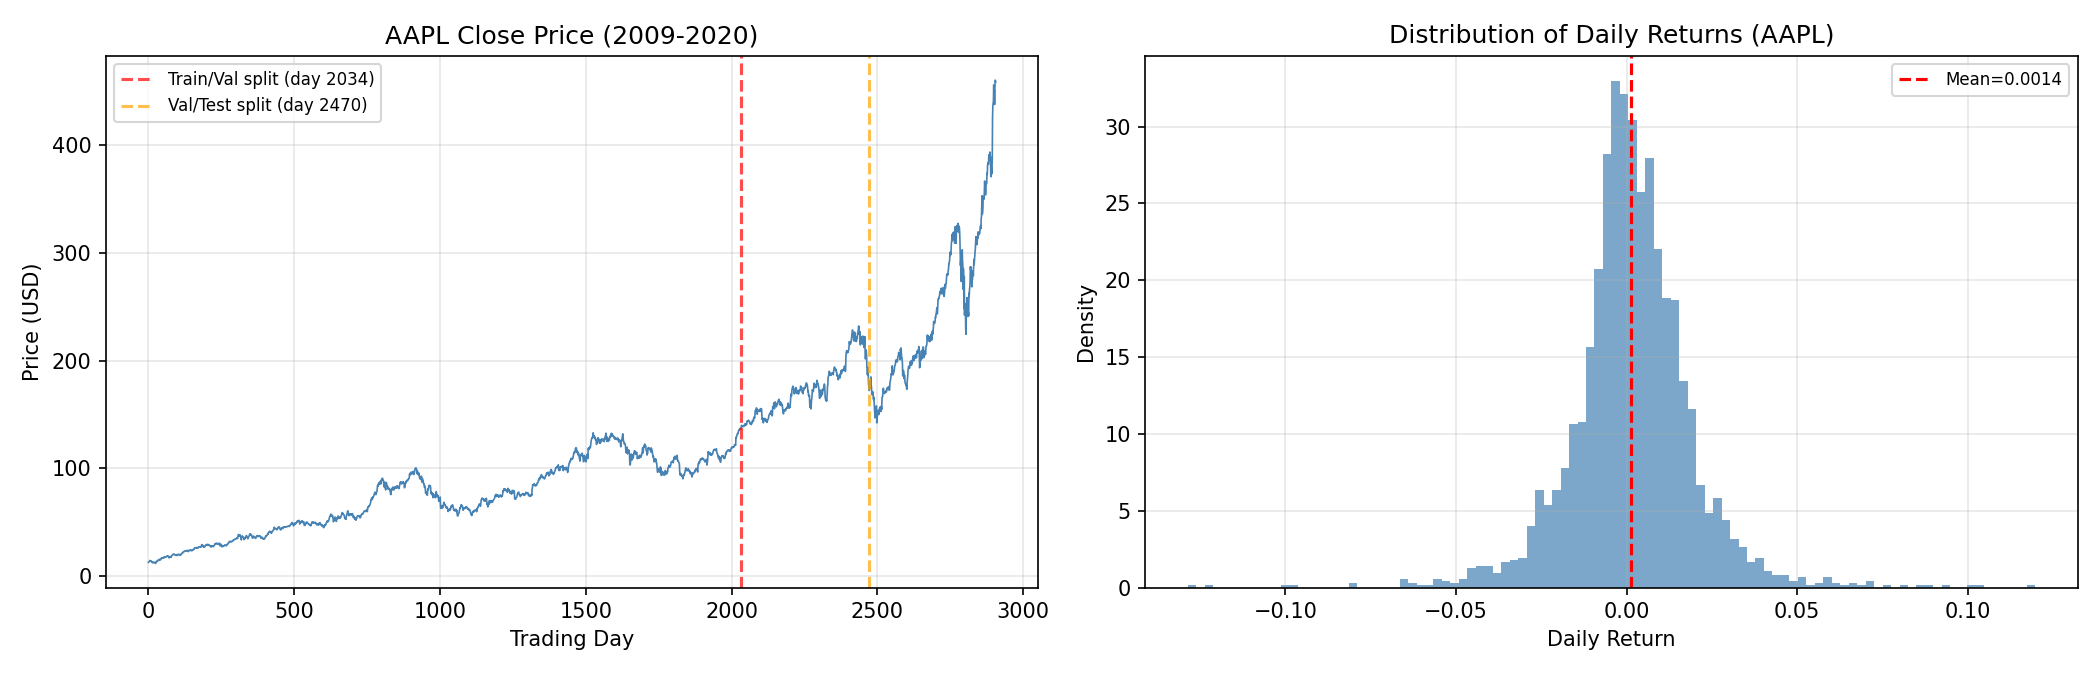
\includegraphics[width=0.95\textwidth]{results/data_exploration.png}
  \caption{Left: AAPL close price (2009--2020) with train/val/test boundaries. Right: Daily return distribution showing fat tails.}
  \label{fig:data}
\end{figure*}

Figure~\ref{fig:corr} shows the Pearson correlation between all 9 features. Most pairs exhibit low correlation, confirming that each indicator captures distinct market signals. The strongest correlations are between BB Width and ATR (0.63), which is expected as both measure volatility, and between the two MA deviations (0.45).

\begin{figure}[H]
  \centering
  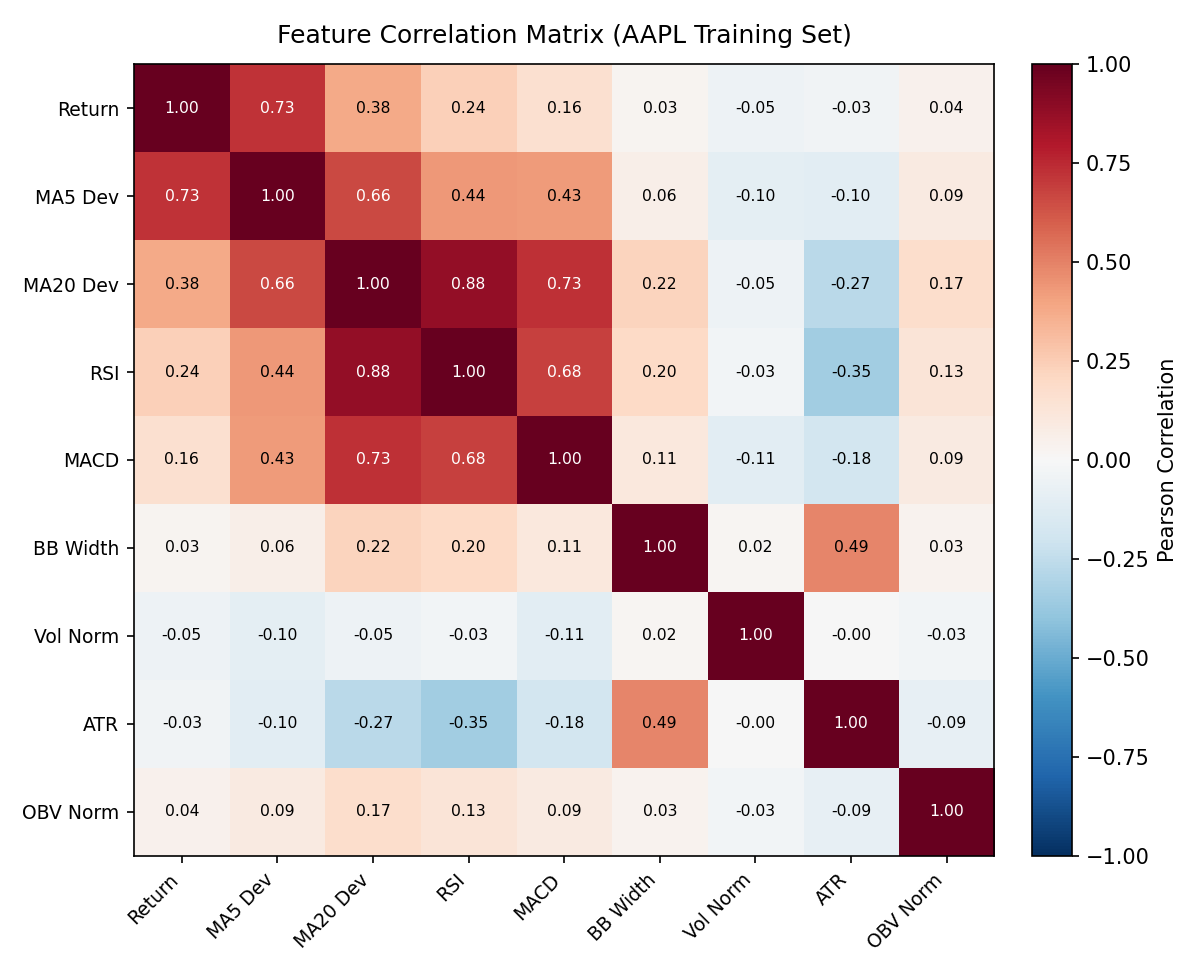
\includegraphics[width=\columnwidth]{results/feature_correlation.png}
  \caption{Feature correlation matrix on the AAPL training set. Low cross-correlation indicates complementary signals.}
  \label{fig:corr}
\end{figure}

The full technical indicator time series and feature distribution comparisons across splits are provided in Appendix~\ref{app:data} (Figures~\ref{fig:indicators} and~\ref{fig:distributions}).

%====================================================================
\section{Environment Design}
%====================================================================

We implement a Gym-style \texttt{TradingEnv} for single-asset trading.
The state $s_t \in \mathbb{R}^{10}$ consists of 9 normalised features plus the current position $\text{pos}_t \in \{-1, 0, +1\}$.
The agent chooses from three discrete \emph{delta} actions: Decrease ($-1$), Hold ($0$), Increase ($+1$), which increment or decrement the position by one unit, clamped to $[\text{pos}_{\min}, \text{pos}_{\max}]$.
This formulation makes partial transitions natural and prevents abrupt position reversals.

The reward is a log-return with transaction cost and drawdown penalty:
\begin{multline}
  r_t = \log\!\frac{V_t}{V_{t-1}}
      - c_t \cdot \mathbf{1}[\text{pos}_t \neq \text{pos}_{t-1}] \\
      + \lambda \min\!\Bigl(0,\; \frac{V_t - V_t^{\text{peak}}}{V_t^{\text{peak}}}\Bigr)
  \label{eq:reward}
\end{multline}
where $\lambda = 0.5$ and $c_t$ is either a flat fee (10~bps) or proportional to position change magnitude.
Rewards are clipped to $[-1, 1]$ for training stability.
The log-return formulation is numerically stable and scale-invariant across tickers.

Training episodes sample a random 252-day window from the training set, providing diverse market regimes per episode. Validation and test episodes always start at index~0 for reproducibility.
The environment tracks position history, trades, and portfolio value, and computes Sharpe ratio, max drawdown, and trade frequency at episode end.

%====================================================================
\section{Deep Learning Methods}
%====================================================================

\textbf{DQN} approximates $Q^*(s,a)$ with a neural network $Q_\theta$ trained via Huber (smooth-$\ell_1$) TD loss:
\begin{equation}
  \mathcal{L} = \mathbb{E}_{\mathcal{D}} \!\Big[\!
    \text{SmoothL1}\!\big( r + \gamma \max_{a'} Q_{\bar\theta}(s', a'),\; Q_\theta(s, a) \big)
  \Big]
  \label{eq:dqn}
\end{equation}
Key components (all from scratch): replay buffer (50K capacity, batch size 128), soft target network update ($\tau{=}0.005$ per step), and exponential $\varepsilon$-decay from 1.0 to 0.02 with decay constant 20K steps.
Rewards are clipped to $[-1,1]$ before training to bound the TD target.

\textbf{DDQN} decouples action selection from evaluation to reduce overestimation:
\begin{equation}
  y_t = r + \gamma \, Q_{\bar\theta}\!\bigl(s',\; \arg\max_{a'} Q_\theta(s', a')\bigr)
  \label{eq:ddqn}
\end{equation}
DDQN subclasses DQN, changing only the target computation.

\textbf{Architecture.}
Both use a 3-layer MLP: $10 \to 128 \to 64 \to 3$ with ReLU activations, Adam ($\text{lr}{=}5{\times}10^{-4}$), and gradient clipping (max norm 1.0).

%====================================================================
\section{Baselines}
%====================================================================

We compare the RL agents against two classical baselines evaluated on the same test set.

\textbf{Buy-and-Hold (B\&H).}
The simplest passive strategy: buy at the start of the test period and hold until the end.
It captures the full market trend and serves as the primary benchmark.

\textbf{ARIMA(1,0,0) walk-forward.}
At each test step $t$ we fit an AR(1) model on a rolling window of the most recent 252 daily returns (using training and validation history as a warm-up) and forecast the next return $\hat{r}_{t+1}$.
The position is set to $+1$ (long) if $\hat{r}_{t+1} > 0$ and $0$ (flat) otherwise, matching the long-only constraint used during RL training.
This baseline tests whether simple autoregressive structure in returns already yields useful trading signals.

\textbf{Momentum (20-day).}
At each test step the trailing 20-day cumulative return is computed as a directional signal.
A positive trailing return triggers a long position; otherwise the agent stays flat.
Momentum is a classic factor in financial economics and a standard weak baseline for active strategies.

\textbf{Random Forest.}
A \texttt{RandomForestClassifier} (200 trees) is trained on the full training+validation set, using the 9 z-score-normalised features to predict the binary sign of the next day's return.
On the test set, a predicted upward day yields a long position; a predicted downward day yields a flat position.
This baseline measures whether a supervised learning approach on the same feature set can outperform the RL agents.

%====================================================================
\section{Training and Results}
%====================================================================

Each agent trains for 200 episodes, each sampling a random 252-day window from the training set (2034 days) to expose the agent to diverse market regimes. Validation uses a deterministic greedy rollout (pure exploitation, from day~0) every 10 episodes; the checkpoint with the best validation score (cumulative return, then Sharpe) is restored for final test evaluation. DQN shows a clear reduction in training loss over time; DDQN convergence is noisier due to more conservative Q-value estimates.

\begin{figure*}[t]
  \centering
  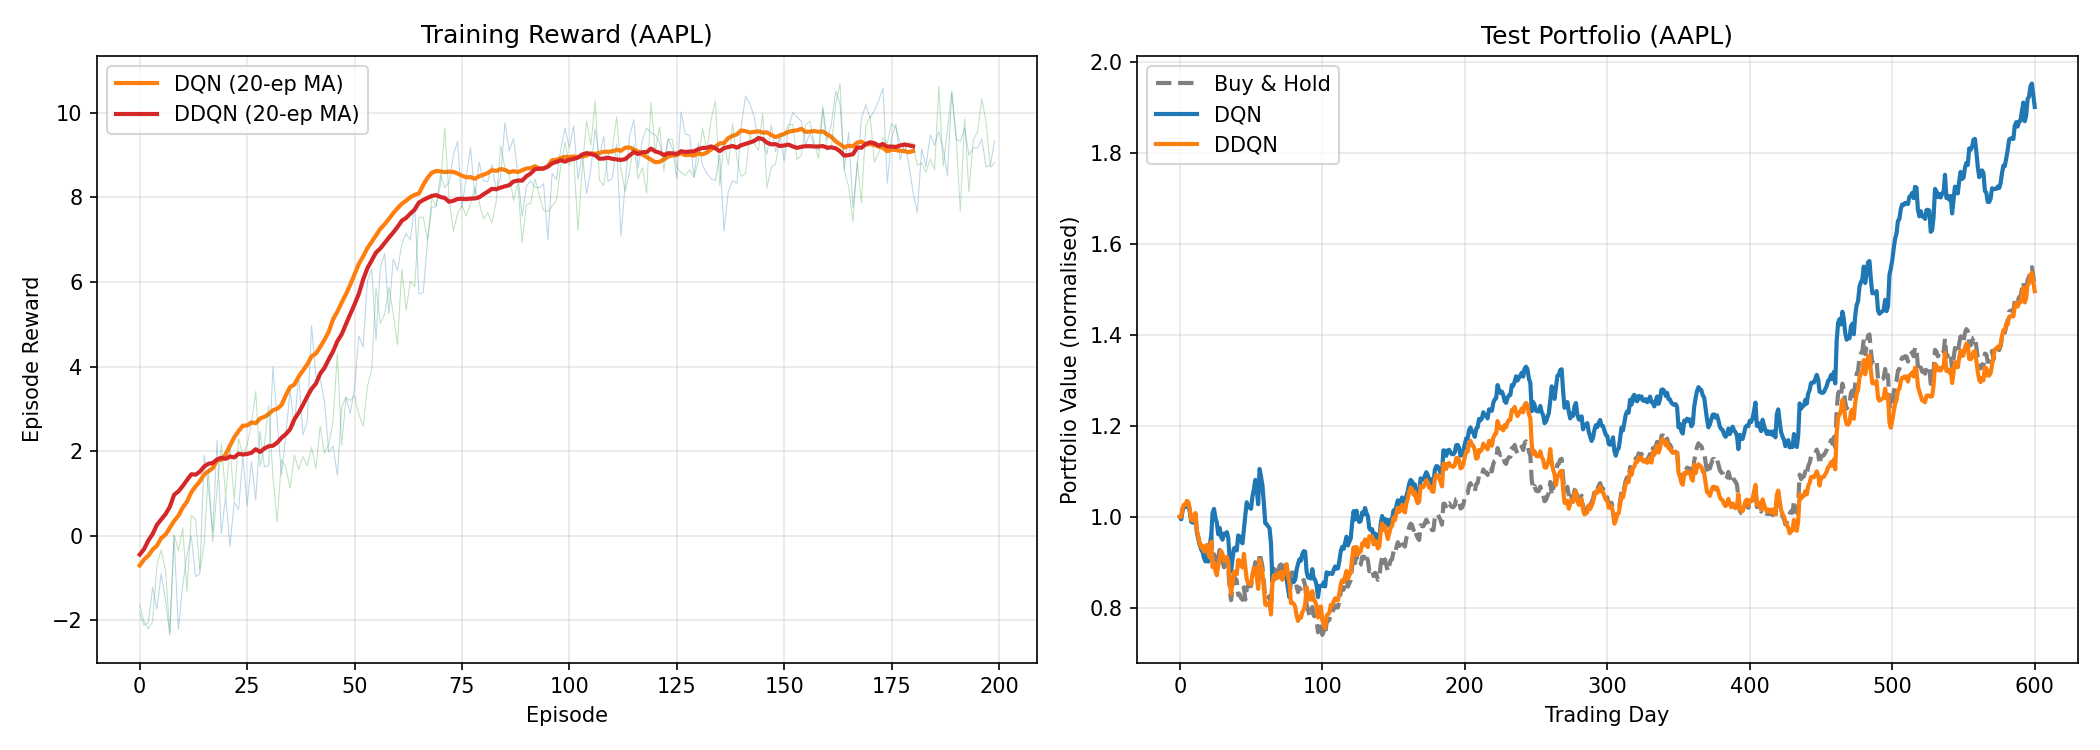
\includegraphics[width=0.95\textwidth]{results/results_AAPL.png}
  \caption{Left: Training reward (20-episode moving average). Right: Test portfolio value for DQN, DDQN, buy-and-hold, and ARIMA baseline.}
  \label{fig:training}
\end{figure*}

\begin{table}[H]
\centering
\caption{Test performance on AAPL (437 days, 2018--2020). ARIMA and agent numbers will be updated after retraining with the revised codebase.}
\label{tab:results}
\begin{tabular}{lccccc}
\toprule
 & \textbf{DQN} & \textbf{DDQN} & \textbf{B\&H} & \textbf{ARIMA} & \textbf{Momentum} & \textbf{RF} \\
\midrule
Cum.\ Return   & +49.6\%   & $-$6.7\%  & +159.0\% & --- & --- & --- \\
Sharpe          & 0.84      & 0.03      & 1.65     & --- & --- & --- \\
Max DD          & $-$32.4\% & $-$38.7\% & $-$31.4\% & --- & --- & --- \\
\bottomrule
\end{tabular}
\end{table}

A detailed episode walkthrough showing position decisions, cumulative reward, and trade markers is provided in Appendix~\ref{app:results} (Figure~\ref{fig:walkthrough}).

The test period (2018--2020) includes the COVID-19 market crash of early 2020, making it a severe out-of-sample stress test.
Buy-and-hold benefits strongly from AAPL's long-term appreciation (${\sim}3\times$ over the period), which is difficult to replicate through active trading.
DQN achieves a positive cumulative return of +49.6\% but falls short of the buy-and-hold baseline, suggesting the agent partially learns to avoid the worst drawdowns but cannot fully capture the sustained uptrend.
DDQN underperforms, ending with a slight loss; its conservative Q-value estimates lead to excessive caution and missed long positions during the recovery.
Both agents exhibit higher max drawdown than buy-and-hold, indicating the reward shaping was insufficient to fully protect against the sudden crash.
These results highlight a fundamental challenge in RL-based trading: a strong passive baseline driven by secular growth is hard to beat with short-horizon signals alone.

%====================================================================
\section{Challenges}
%====================================================================

An early bug used normalised returns (std${\approx}1$) instead of raw returns for rewards, producing unrealistic values; fixed by separating \texttt{raw\_return}.
Initial linear $\varepsilon$-decay exhausted exploration too quickly; switched to exponential decay for smoother exploration–exploitation trade-off.
MSE loss was sensitive to large reward outliers; replaced with Huber (smooth-$\ell_1$) loss and added reward clipping to $[-1,1]$.
Hard target-network copies caused training instability; replaced with soft polyak updates ($\tau{=}0.005$).
Short-selling can cause portfolio values below zero, so we clamp at $10^{-8}$.

%====================================================================
\section{Future Work}
%====================================================================

Extensions include policy gradient methods (PPO) for continuous position sizing, multi-asset portfolio environments, LSTM architectures for temporal dependencies, and Sharpe/CVaR-based reward formulations.

%====================================================================
\section{Contributions}
%====================================================================

\begin{table}[H]
\centering
\small
\begin{tabular}{p{0.18\columnwidth} p{0.72\columnwidth}}
\toprule
\textbf{Member} & \textbf{Contributions} \\
\midrule
Rutwik &
DQN/DDQN implementation from scratch; hyperparameter tuning (lr, batch size, buffer size); exponential $\varepsilon$-decay; soft target-network updates ($\tau{=}0.005$); Huber loss and reward clipping; position-delta action space; log-return reward; random episode windows; best-model checkpointing; baseline comparison integration \\
\midrule
Yufan &
Data pipeline: \texttt{yfinance} OHLCV download, 9-feature engineering (RSI, MACD, Bollinger Bands, ATR, OBV, configurable MA deviations, volume normalisation), train-only z-score normalisation, multi-ticker \texttt{load\_all()} support.
\texttt{TradingEnv}: drawdown-penalised reward shaping (Eq.~\ref{eq:reward}), flat \& proportional transaction cost models, built-in Sharpe/drawdown/trade-frequency evaluation, position and portfolio tracking, episode logic \\
\midrule
Fei Xin &
Evaluation framework, training visualisation, report, and slides \\
\bottomrule
\end{tabular}
\end{table}

%====================================================================
\begin{thebibliography}{9}
\bibitem{mnih2015}
V.~Mnih et al., ``Human-level control through deep reinforcement learning,'' \emph{Nature}, 518:529--533, 2015.
\bibitem{hasselt2016}
H.~van Hasselt et al., ``Deep reinforcement learning with double Q-learning,'' \emph{AAAI}, 2016.
\bibitem{yang2020}
H.~Yang et al., ``Deep reinforcement learning for automated stock trading: An ensemble strategy,'' \emph{ACM ICAIF}, 2020.
\end{thebibliography}

%====================================================================
\appendix
\onecolumn

%====================================================================
\section{Data Pipeline Visualisations}
\label{app:data}
%====================================================================

\begin{figure}[H]
  \centering
  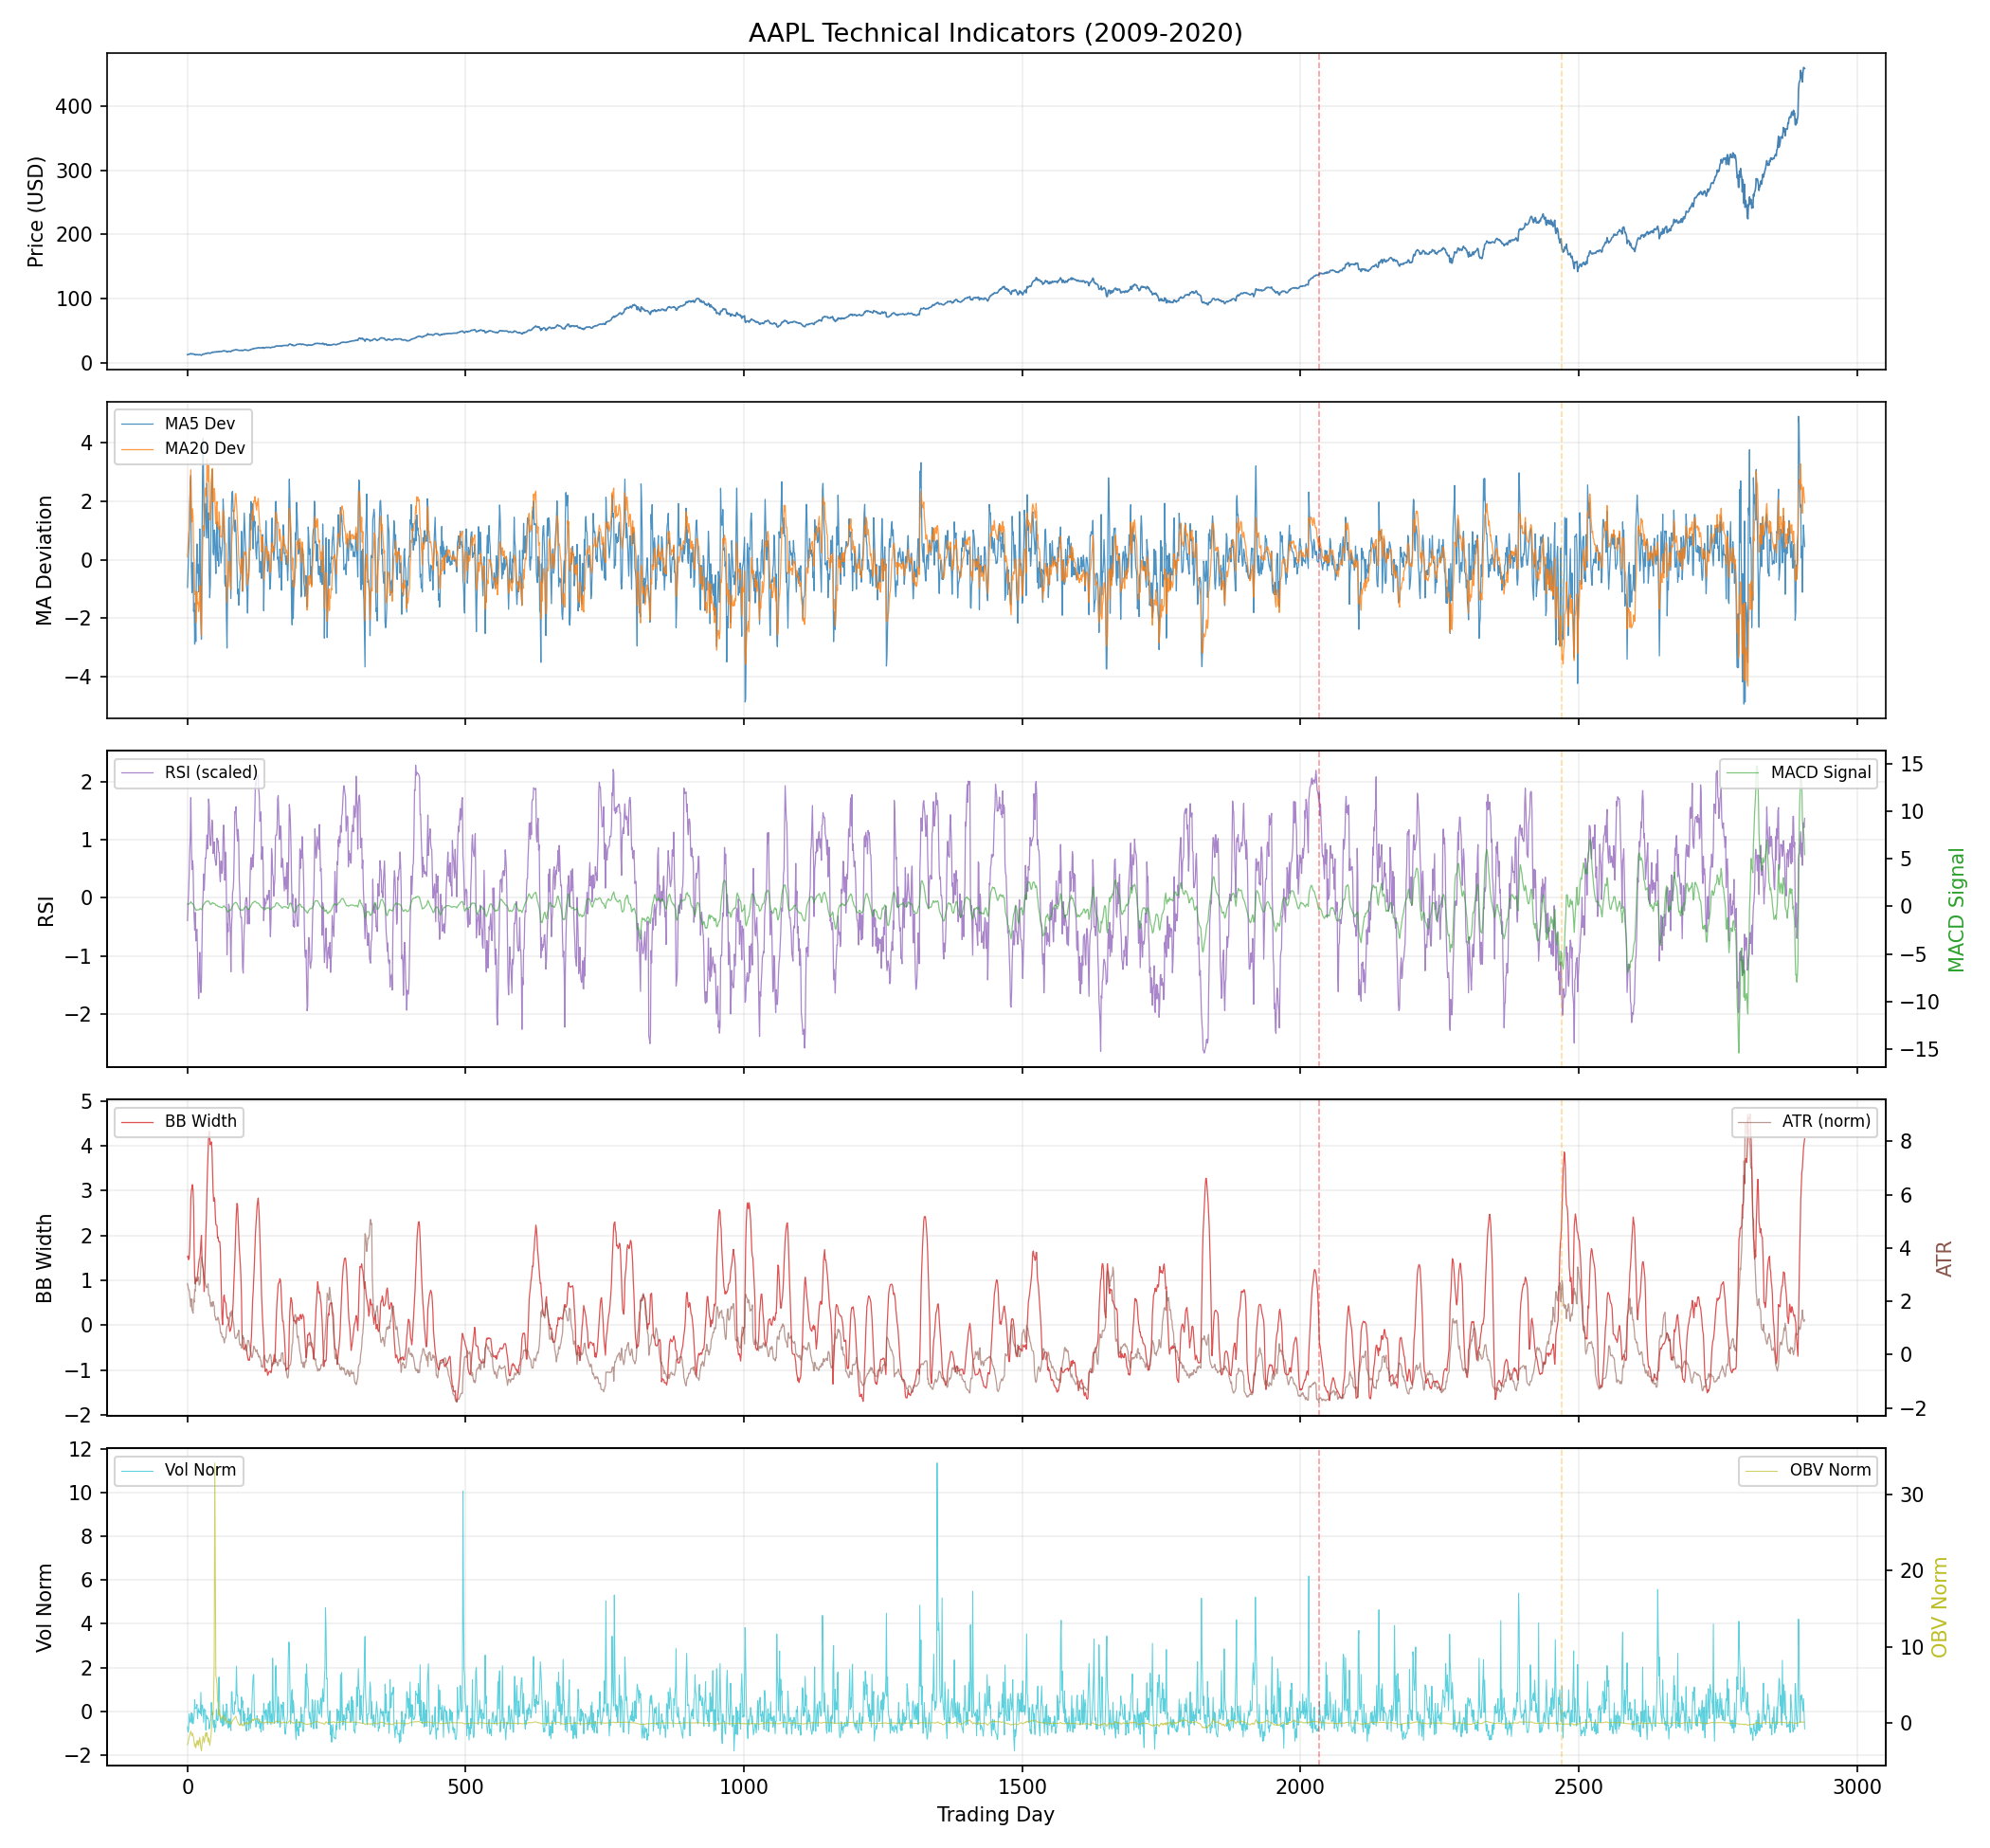
\includegraphics[width=0.95\textwidth]{results/technical_indicators.png}
  \caption{Technical indicator time series for AAPL (2009--2020). From top: close price, MA deviations, RSI \& MACD, Bollinger width \& ATR, volume \& OBV. Dashed lines mark train/val/test boundaries.}
  \label{fig:indicators}
\end{figure}

\begin{figure}[H]
  \centering
  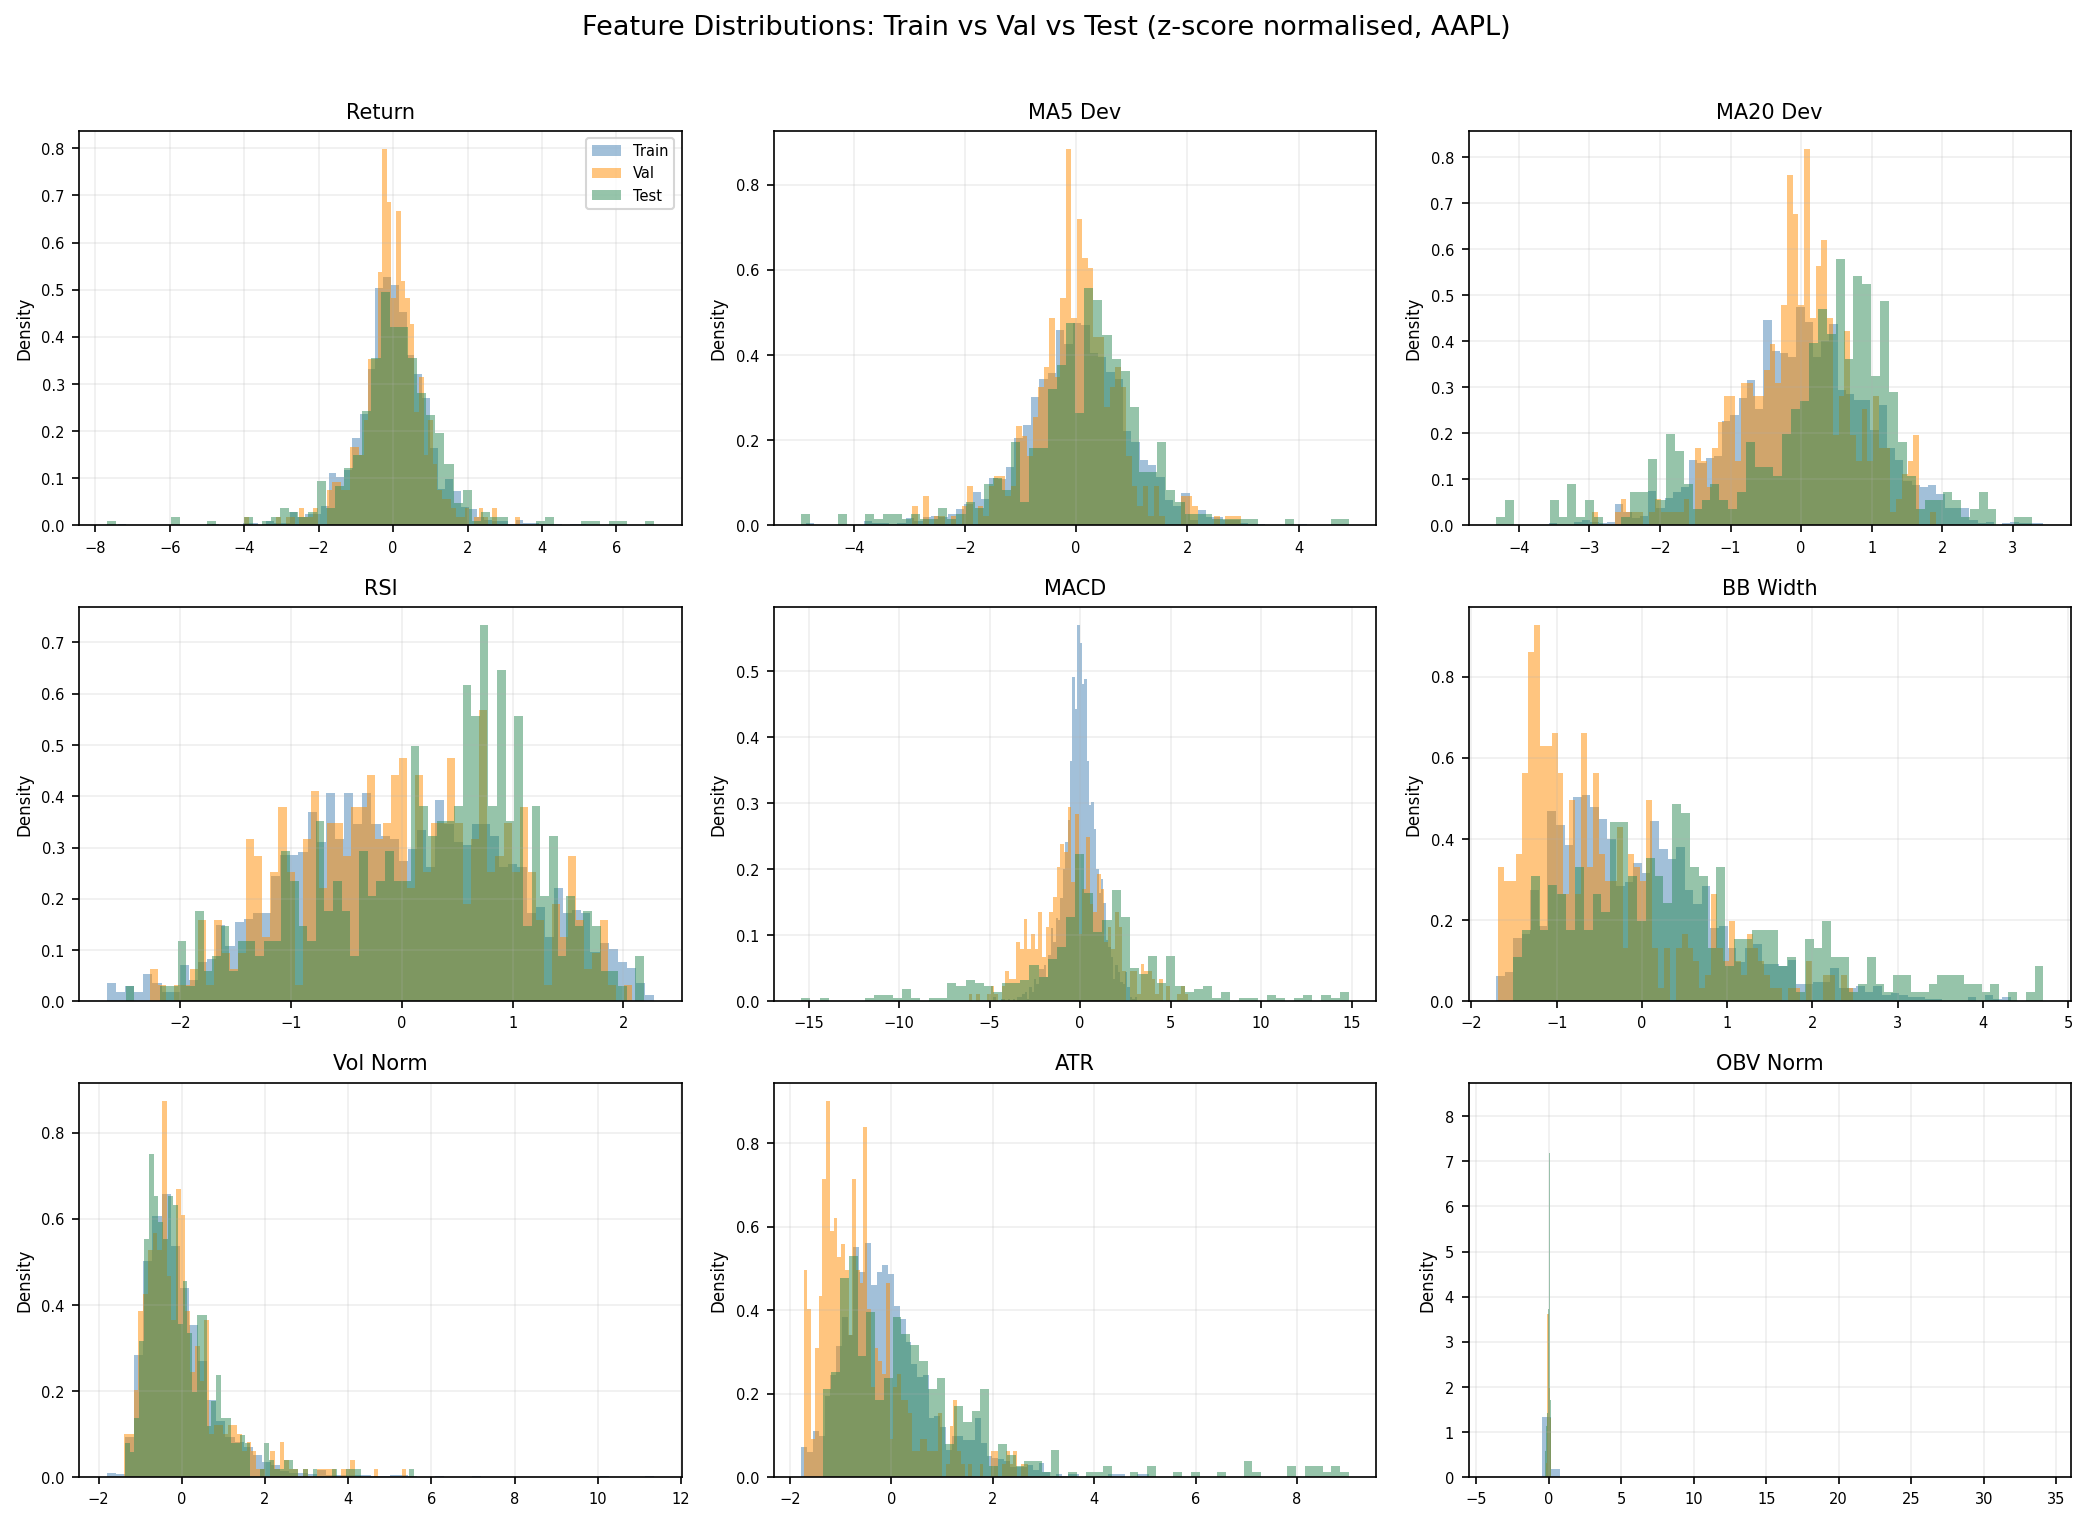
\includegraphics[width=0.95\textwidth]{results/feature_distributions.png}
  \caption{Feature distributions across train/val/test splits (z-score normalised using training-set statistics only). Overlapping distributions confirm consistent normalisation without look-ahead bias.}
  \label{fig:distributions}
\end{figure}

%====================================================================
\section{Episode Walkthrough}
\label{app:results}
%====================================================================

\begin{figure}[H]
  \centering
  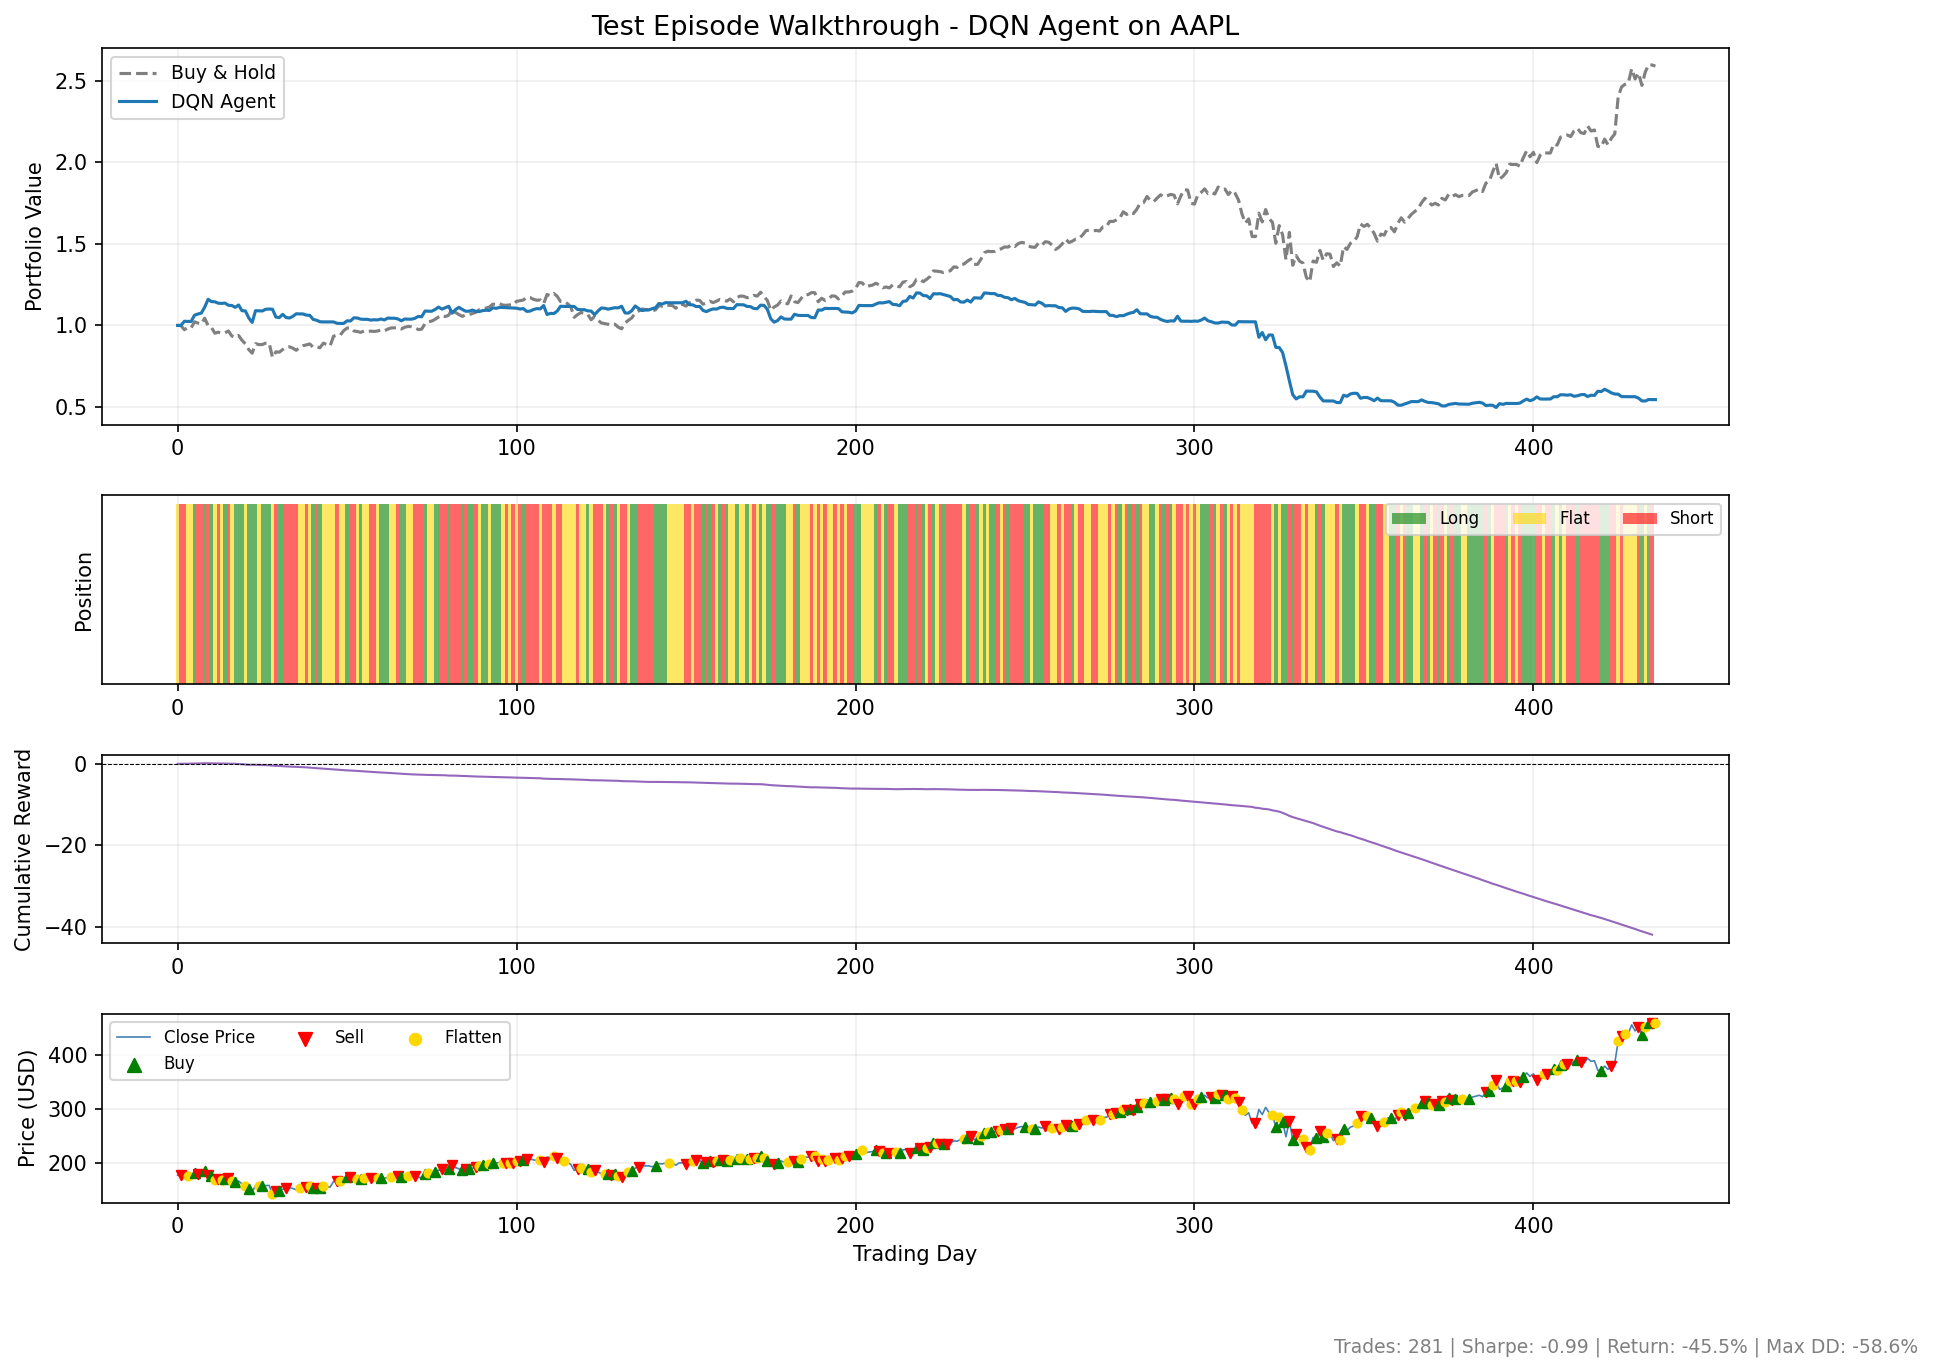
\includegraphics[width=0.95\textwidth]{results/episode_walkthrough.png}
  \caption{DQN test episode walkthrough on AAPL. Top: portfolio value vs buy-and-hold. Second: position colour bands (green=long, gold=flat, red=short). Third: cumulative reward. Bottom: buy/sell markers on close price.}
  \label{fig:walkthrough}
\end{figure}

\end{document}
